% vim: set spelllang=fr:
\chapter{Annotation en rôles sémantiques fondée sur la connaissance}
\label{ch:srl}


%\citep{simmons1973semantic} is the earliest work on Semantic Role Labeling.
%Already based on \citep{fillmore1968case}, it parsed a sentence into what we
% know call semantic roles. (check)

%Contrairement aux autres ressources pour l'annotation en rôles sémantiques,
%VerbNet couvre l'ensemble des verbes fréquents du vocabulaire tout en étant
%conçu sur des préceptes robustes le rendant utile pour les tâches de Traitement
%Automatique des Langues (Section~\ref{ch:verbnet:sec:verbnet}).

La tâche d'annotation en rôles sémantiques a reçu beaucoup d'attention ces
dernières années, à la fois pour les approches supervisées et semi-supervisées.
Les approches fondées sur la connaissance, elles, ne se basent pas sur des
corpus annotés mais sur des ressources lexicales existantes. Ce type d'approche
a été négligé malgré leur complémentarité par rapport aux autres approches.

En nous inspirant de \citep{swier2004unsupervised,swier2005exploiting}, nous
présentons dans ce chapitre un système d'annotation en rôles sémantiques fondé
sur la connaissance qui se veut simple à mettre en place et facile à
reproduire. La prise en compte de divers phénomènes linguistiques doit
permettre d'améliorer les performances par rapport à un état donné. Par
exemple, la prise en compte de la voix passive a réduit le taux d'erreur de
15,7~\%, ce qui montre la marge de progrès existante. Malgré des performances
moindres par rapport aux approches supervisées quand des données d'entraînement
existent, l'approche facilite l'analyse des erreurs, n'a pas besoin d'un corpus
annoté manuellement et est \textit{a priori} indépendante du domaine considéré.

Ce chapitre se concentre sur notre système d'annotation en rôles sémantiques
dans un cadre général en l'utilisant sur le corpus FrameNet anglais (qui a été
présenté à la section~\ref{presentation_framenet}). Le chapitre suivant
montreront la versatilité de ce système dans des contextes différents : en
domaine spécifique avec les domaines du football, du réchauffement climatique
et de l'informatique en anglais et en français (Chapitre~\ref{ch:domainsrl}).
Ce chapitre est une réécriture complète de travaux déjà publiés
\citep{pradet2013revisiting}.

\section{Tâche}

L'objectif de ce chapitre est de présenter notre système en l'évaluant sur une
conversion VerbNet du corpus annoté en rôles sémantiques fourni par FrameNet,
ce qui permet d'évaluer l'annotation en rôles sémantiques VerbNet. La
figure~\ref{fig:srlrussia} est un exemple d'annotation en rôles sémantiques
avec des frames et des rôles FrameNet. Nous utiliserons notamment cette phrase
d'exemple par la suite pour illustrer notre propos. Pour une phrase donnée, les
prédicats verbaux et la frame qu'ils évoquent sont identifiés. Dans chaque
phrase, des syntagmes vont remplir un des rôles prévus par la frame dans
FrameNet. Ces syntagmes sont nommés «~remplisseurs de rôle~» (\textit{role
filler} en anglais).

\begin{figure}[ht]
    La phrase à annoter est :

    \begin{quote}
    However, in 2002 Russia declared it will eliminate its tactical nuclear weapons by the end of 2004.
    \end{quote}

    L'objectif est d'aboutir à la représentation suivante :

    \begin{itemize}
        \item \textit{declare} déclenche la frame Statement dont les rôles sont remplis ainsi :
        \begin{itemize}
            \item Speaker : Russia
            \item Message : it will eliminate its tactical nuclear weapons by the end of 2004
            \item Time : in 2002
        \end{itemize}
        \item \textit{eliminate} déclenche la frame Removing dont les rôles sont remplis ainsi :
        \begin{itemize}
            \item Agent: it
            \item Theme: its tactical nuclear weapons
            \item Source: \textit{non instancié}
        \end{itemize}
    \end{itemize}
    \caption{\label{fig:srlrussia}Exemple d'annotation en rôles sémantiques}
\end{figure}

Toute interprétation supplémentaire non présente dans la
figure~\ref{fig:srlrussia} est en dehors du cadre de l'annotation en rôles
sémantiques, ce qui est la raison pour laquelle la tâche est aussi connue sous
le nom d'analyse sémantique de surface (\textit{shallow semantic parsing}).  Il
est néanmoins intéressant de garder à l'esprit les applications possibles de
tels travaux. Par exemple, un système de question-réponse pourrait utiliser la
représentation de ces deux \textit{frames} pour répondre à la question \textit{Does
Russia possess tactical nuclear weapons?} L'annotation de la
figure~\ref{fig:srlrussia} est une information utile, mais elle ne serait pas
suffisante pour répondre à la question : il faut aussi comprendre la question,
annoter les coréférences (\textit{it} fait référence à \textit{Russia}), comprendre
la sémantique \textit{Removing}, établir la crédibilité du \textit{Speaker},
s'intéresser à d'autres phrases potentiellement contradictoires, etc.

\section{Système}

Le système présenté est similaire à celui de
\cite{swier2004unsupervised,swier2005exploiting} qui se base sur VerbNet.
Néanmoins, les ressources utilisées ont beaucoup progressé (VerbNet 1.5 contre
VerbNet 3.2 notamment). Les corpus sur lesquels s'évaluer ont aussi évolué. En
particulier, les systèmes basés sur FrameNet n'utilisent plus le corpus de
phrases d'exemples choisis pour leur diversité syntaxique mais s'évaluent sur
des annotations de toutes les frames présentes dans des textes issus de
différentes sources. \cite{swier2005exploiting} utilisent aussi un mapping non
disponible alors que le projet SemLink a fourni un mapping FrameNet-VerbNet
«~officiel~». Dix ans après, il est donc important d'évaluer à nouveau cette
approche pour savoir où elle se situe par rapport à l'état de l'art. Nous
proposons par ailleurs certaines améliorations.

Pour commencer, chaque phrase à annoter doit d'abord être étiquetée en
morphosyntaxe et analysée syntaxiquement. Nous laissons ici ces analyses à des
systèmes externes présentés à la section~\ref{subsec:details_exp}. Ces analyses
sont l'entrée de notre système, la sortie étant l'annotation en rôles
sémantiques montrée dans la figure~\ref{fig:srlrussia}.

Ensuite, nous utilisons les informations de VerbNet (présenté à la
section~\ref{presentation_verbnet}) sur l'interface entre la syntaxe
et la sémantique. Dans VerbNet, chaque classe regroupe un certain nombre de
verbes acceptant tous les mêmes constructions syntaxiques. Les syntagmes
participant à ces constructions sont associés à des rôles sémantiques à
interpréter dans le contexte de la classe. Ces \textit{frames} sont notées de
cette façon : NP.Agent V NP.Theme. Ici, dans cette construction transitive
(NP V NP, e.g. \textit{Sally pushed the chair}), le premier syntagme nominal
(\textit{Sally}) est Agent alors que le second (\textit{the chair}) est Theme.
Bien que des règles précises régissent leur attributions, l'interprétation
complète des rôles (ici Theme et Agent) dépend de la classe VerbNet
considérée. Par exemple, la classe \texttt{resign-10.11} contient notamment
NP.Agent V PP.Source (\textit{I resigned from the military}). Dans cette
classe, l'Agent est la personne qui démissionne et la Source est le poste qui
a été quitté.

Pour une phrase donnée, le système commence par identifier les verbes de cette
phrase. Pour chacun de ces verbes, un ensemble de classes VerbNet est
identifié. Ainsi, pour notre phrase d'exemple ci-dessus, les classes possibles
pour le verbe \textit{declare} sont \texttt{declare-29-4-1-1-1},
\texttt{say-37.7-1} et \texttt{reflexive\_appearance-48.1.2}. Le choix correct
est \texttt{say-37.7-1}, mais il ne nous est pas possible de le déterminer
avant de considérer les frames listées par VerbNet dans ces différentes
classes.

Par exemple, \texttt{reflexive\_appearance-48.1.2} contient la frame NP.Agent V
NP.Theme. Ainsi, si un des verbes de cette classe, tel que \textit{present} :
\begin{itemize}
    \item est utilisé dans un sens compatible avec la classe
        \texttt{reflexive\_appearance-48.1.2},
    \item et est utilisé avec un sujet syntagme nominal et un objet syntagme
        nominal,
\end{itemize}
alors le sujet du verbe est l'Agent et l'objet est le Theme.

La phrase d'exemple de la figure~\ref{fig:srlrussia} ne correspond pas à NP V
NP mais à NP V that S (\textit{that S} étant la notation VerbNet pour les
complétives introduites par \textit{that}). La seule occurrence de cette frame
VerbNet est dans \texttt{say-37.7-1} : NP.Agent V that S.Topic (\textit{He
ordered that he go}). Les classes \texttt{declare-29-4-1-1-1} et
\texttt{reflexive\_appearance-48.1.2} ne listant pas cette frame, il est
possible d'établir que :

\begin{itemize}
    \item la classe VerbNet qui convient est \texttt{say-37.7-1},
    \item \textit{Russia} est Agent,
    \item \textit{it will eliminate its tactical nuclear weapons by the end of 2004} est Topic.
\end{itemize}

% TODO la conversion se fait dans l'autre sens
Enfin, le mapping entre VerbNet et FrameNet (section~\ref{subsec:mapping}) nous
informe que :

\begin{itemize}
    \item la classe VerbNet \texttt{say-37.7} correspond à la frame Statement,
    \item dans cette classe, le rôle VerbNet Agent correspond au rôle FrameNet Speaker,
    \item dans cette classe, le rôle VerbNet Topic correspond au rôle FrameNet Topic.
\end{itemize}

Nous aboutissons ainsi à l'annotation en rôles sémantiques voulue pour notre
phrase d'exemple.

On ne peut pas toujours identifier la classe VerbNet correcte. C'est le cas par
exemple de \texttt{reflexive\_appearance-48.1.2} et \texttt{say-37.7-1} qui
contiennent toutes les deux le cadre NP V NP. Ainsi, si notre phrase d'exemple
avait été \textit{Russia declared its intentions}, la classe serait restée
ambigüe. Sans corpus annoté, ces ambiguïtés ne peuvent pas être résolues.
Cependant, une fois qu'une première série de correspondances a été effectuée,
il est possible d'utiliser les connaissances du domaine étudié pour annoter de
nouveaux syntagmes nominaux (section~\ref{subsec:probability}).

Alors que nous avons jusqu'ici décrit le déroulement général du système afin
d'en donner l'intuition, les sections suivantes expliquent le déroulement
précis du système qui est découpé en quatre étapes.

\subsection{Identification du prédicat}

Chaque phrase peut contenir un ou plusieurs prédicats : nous nous contentons
ici de retenir tous les verbes présents dans VerbNet. Les autres prédicats
potentiels, c'est-à-dire ceux qui ne sont pas dans VerbNet et ne sont pas des
verbes, sont ignorés. Les parties du discours acceptées sont toutes celles
concernant des verbes : md, MD, VB, VBD, VBG, VBN, VBP, VBZ, VV, VVD, VVG, VVN,
VVP, VVZ, VH, VHD, VHG, VHN, VHP et VHZ.
% TODO la liste est différente dans argguesser.py/argheuristic.py
% TODO en annexe !

\subsection{Identification des arguments}

% TODO 80% Das + http://www.aclweb.org/anthology/I/I13/I13-1094.pdf ?

% TODO tagset syntaxique WSJ
Cette étape identifie les syntagmes amenés à jouer un rôle sémantique lors de
l'annotation. Nous suivons ici \cite{lang2011unsupervised} qui propose huit
règles\footnote{La septième règle n'est pas utilisée.} basées sur l'analyse
syntaxique de la phrase. Initialement, tous les mots sont candidats. Puis
chacune de ces règles sélectionne ou écarte des mots candidats. Dans la
représentation en dépendances, si le mot sélectionné est la tête d'un syntagme,
c'est le syntagme entier qui devient candidat. Sinon, c'est uniquement le mot.
Voici les règles appliquées dans l'ordre :

\begin{enumerate}
    \item Éliminer les déterminants, les marqueurs d'infinitifs, les conjonctions de coordinations et la ponctuation.
    \item Éliminer les candidats dont le chemin du prédicat au candidat finit par une coordination, une subordination, etc.
    \item Conserver les candidats qui sont les sujets les plus proches à gauche du prédicat et dont les relations du prédicat p à la tête t du candidat sont toutes montantes (t $\rightarrow$ p).
    \item Éliminer les candidats  dont le chemin entre le prédicat et le candidat, sauf la dernière relation, contient une relation de sujet, une relation de modifieur adjectival, etc.
    \item Éliminer les verbes auxiliaires.
    \item Conserver les candidats directement sous le prédicat.
    \item \sout{Conserver les candidats si le chemin du prédicat au candidat traverse plusieurs noeuds verbaux.}
    \item Éliminer tous les candidats restants.
\end{enumerate}

% TODO exemple
Pour les règles 3 et 4, la liste complète des relations acceptées est donnée en
annexe à la section~\ref{argument_identification}. En pratique, sur le corpus
FrameNet, ces règles génèrent les candidats valides mais aussi certains qui ne
jouent pas de rôle : notre système devra par la suite pouvoir écarter ces
candidats tout en assignant les rôles corrects aux candidats qui jouent bien un
rôle.

Cette étape d'identification des arguments est facultative : afin de mieux
comprendre les performances des étapes suivantes, ce seront parfois les
arguments parfaits de la vérité-terrain qui seront utilisés lors de
l'évaluation. En effet, l'objectif est d'évaluer l'apport de VerbNet à la tâche
de l'annotation en rôles sémantiques, et l'identification des arguments, bien
qu'une partie intégrante de tout système complet d'annotation en rôles
sémantiques \citep{das2010probabilistic}, ne fait pas partie de nos
contributions.

\subsection{Correspondance exacte des frames}

Cette étape associe zéro, un ou plusieurs rôles sémantiques à chaque syntagme
candidat identifié lors de l'étape précédente. Elle correspond au \textit{frame
matching} de \citet{swier2005exploiting}.

Nous incluons ici deux étapes traditionnellement séparées dans les systèmes
d'annotation en rôles sémantiques : l'identification des frames FrameNet puis
l'assignation de rôles aux arguments précédemment identifiés
\citep{gildea2002automatic,das2014frame}. Nous commençons ici par identifier
les frames VerbNet possibles pour restreindre au maximum le nombre de classes
VerbNet applicables ; le but étant de n'en avoir qu'une. En effet, même si
toutes les classes VerbNet réutilisent les mêmes rôles, le sens précis d'un
rôle est déterminé par la classe qu'il faut donc identifier.

Regardons comment se déroule cette étape. Premièrement, les syntagmes candidats
sont représentés au format VerbNet. Par exemple, si trois syntagmes nominaux
ont été identifiés comme arguments, dont un avant le verbe, la représentation
VerbNet de la phrase devient NP V NP NP. Si le troisième syntagme est un
syntagme prépositionnel introduit par \textit{in}, la représentation devient NP
V NP in PP, et ainsi de suite.

Ensuite, pour comparer la représentation VerbNet de la phrase aux frames
VerbNet, nous identifions toutes les classes VerbNet incluant le prédicat. Par
exemple, le prédicat \textit{classify} est présent dans deux classes VerbNet~:
\texttt{characterize-29.2} et \texttt{classify-29.10}. Les frames VerbNet
possibles sont~:

% TODO séparer par classe, on doit pouvoir suivre la suite sans regarder
% VerbNet
\begin{itemize}
    \item NP.Agent V NP.Theme (as) S\_ING.Attribute
    \item NP.Agent V NP.Theme to be ADJ.Attribute
    \item NP.Agent V NP.Theme as PP.Attribute
    \item NP.Agent V NP.Theme
    \item NP.Agent V NP.Theme as PP.Goal
    \item NP.Agent V NP.Theme in PP.Location
\end{itemize}
% TODO documenter la gestion des PP - demande de savoir comment on unifie avec
% domainsrl

% TODO commencer par la phrase d'exemple (declare ou eliminate)
Considérons la phrase \textit{The curator classified the artifacts}. La
représentation VerbNet de cette phrase est NP V NP, ce qui correspond au
NP.Agent V NP.Theme de la classe \texttt{classify-29.10}. On en déduit que
\textit{The curator} est Agent, et que \textit{the artifacts} est Theme. Cette
phrase est donc correctement annotée en rôles sémantiques VerbNet.

Prenons un autre example, cette fois tiré de FrameNet. La phrase \textit{The
company also classifies short and wide radius ruts according to their severity}
est transformée en NP V NP according PP. Dans ce cas, seuls les deux premiers
syntagmes peuvent être mis en correspondance avec les frames VerbNet listées
ci-dessus. Il n'y a pas de correspondance possible pour le troisième syntagme:
VerbNet n'encode pas \textit{according} comme une préposition possible alors que
\textit{in} et \textit{as} sont acceptées. De tels arguments non prévus pas VerbNet
ne sont pas annotés lors de cette étape. C'est ici un problème de couverture.
Les auteurs de VerbNet travaillent actuellement sur la couverture de la
ressource en ajoutant des informations syntaxiques et lexicales issues de très
larges corpus \citep{bonial2013expanding}. Le résultat de ces travaux n'est
cependant pas disponible dans la version 3.2 de VerbNet que nous utilisons. Ce
problème de couverture empêche d'assigner la classe VerbNet qui convient. Par
conséquent, même si on sait que quelle que soit la classe, le sujet serait
Agent et le premier objet Theme, cette information est difficilement
interprétable dans une application.

% TODO différents algorithmes de match
% TODO nouvel algorithme : oublier complètement l'ordre

%Une autre difficulté fréquente en français est l'ordre des objets du verbe.
%Prenons les phrases suivantes, inspirées de la classe \texttt{cut-21.1} :

%\begin{itemize}
%    \item \textit{Luc a découpé la photo dans le journal avec des ciseaux}
%    \item \textit{Luc a découpé avec des ciseaux la photo sa maison de vacances dans le journal de la commune de Lacanau}
%    \item\e Luc a découpé avec des ciseaux dans le journal la photo où il montre l'énorme poisson qu'il venaît de pêcher
%\end{itemize}


\subsection{Correspondance probabiliste des frames}
\label{subsec:probability}

Maintenant que les correspondances exactes ont étés effectuées, il reste d'une
part les correspondances impossibles et les correspondances ambigües pour
lesquelles plusieurs frames sont possibles. Alors que les correspondances
impossibles sont à corriger au niveau de la ressource VerbNet ou au niveau de
l'analyse syntaxique, nous pouvons utiliser les frames déjà mises en
correspondance pour désambiguïser les correspondances ambigües. La méthode
reste non supervisée : bien que nous entraînions une forme simple d'algorithme
supervisé, nous le faisons sur des données qui sont initialement non annotées.
En effet, elles sont simplement obtenues automatiquement sur le corpus existant
à l'aide de la correspondance exacte. Nous faisons ici l'hypothèse qu'un corpus
entier est à annoter, mais dans le cas où l'annotation se ferait phrase par
phrase, il serait possible d'abandonner cette étape ou d'alimenter les
classifieurs que nous utilisons au fur et à mesure des annotations. Cette étape
correspond aux \textit{probability models} de \citet{swier2004unsupervised}.

L'apprentissage se fait sous la forme d'un simple classifieur statistique. Deux
classifieurs sont utilisés : le premier détermine la classe VerbNet quand
celle-ci est ambigüe, et le second détermine le rôle d'un syntagme quand
plusieurs choix sont possibles.

Le premier classifieur détermine la classe VerbNet en fonction du prédicat.
\citet{abend2008supervised} ont déjà identifié cette tâche comme étant proche
de la désambiguïsation lexicale. Dans cette tâche, il est difficile de battre
la \textit{baseline} du sens le plus fréquent. Par exemple, lors de la tâche de
désambiguïsation lexicale de SemEval-2007, seuls 25~\% des systèmes ont fait
mieux que cette baseline, et les autres systèmes ont incorporé cette
information. Nous choisissons de rester pour l'instant dans la simplicité en
utilisant directement cette baseline :

$$ \text{classe} = \arg\max_{\text{classe}} p(\text{classe} \vert \text{prédicat}) $$

Le second classifieur (issu de \cite{swier2004unsupervised}) assigne une
probabilité aux différents rôles possibles en s'aidant des rôles déjà
identifiés.

% TODO belles formules comme dans gildea2002automatic
$$ \text{rôle} = \arg\max_{\text{rôle}} p(\text{rôle} \vert \text{prédicat}, \text{fonction})$$

La fonction est la fonction grammaticale identifiée d'après l'analyse
syntaxique : si un syntagme apparaît avant le verbe, il est sujet, s'il est
après le verbe, et il est objet, et ainsi de suite. Les syntagmes
prépositionnels sont traités à part : la préposition qui introduit le syntagme
est considérée à part.

Ce classifieur utilise l'information du prédicat et la fonction grammaticale
détectée. Par exemple, dans notre corpus (section~\ref{subsec:details_exp}),
l'objet direct du verbe \textit{négliger} est le plus souvent \textit{Theme}. La
précision pour ce modèle est forte, mais il n'assigne des rôles que pour 40~\%
des arguments : dans les autres cas, nous ne disposons pas d'informations pour
cette paire (prédicat, fonction grammaticale).

\subsection{Mapping VerbNet - FrameNet}
\label{subsec:mapping}

Le projet SemLink a développé un mapping entre VerbNet et FrameNet. Pour chaque
frame VerbNet, zéro, une ou plusieurs classes FrameNet ont été choisies.
Ensuite, pour chaque paire (VerbNet, FrameNet), les rôles des deux ressources
sont associés.
% TODO et le second fichier qui traite des verbes ?

\begin{figure}[ht]
    \begin{minted}{xml}
    <vncls class='9.1' fnframe='Placing'>
        <roles>
        <role fnrole='Agent' vnrole='Agent'/>
        <role fnrole='Cause' vnrole='Agent'/>
        <role fnrole='Goal' vnrole='Destination'/>
        <role fnrole='Theme' vnrole='Theme'/>
        </roles>
    </vncls>
    <vncls class='9.1-1' fnframe='Installing'> <!-- added for 'install' -->
        <roles>
        <role fnrole='Agent' vnrole='Agent'/>
        <role fnrole='Fixed_location' vnrole='Destination'/>
        <role fnrole='Component' vnrole='Theme'/>
        </roles>
    </vncls>
    <vncls class='9.3' fnframe='Cause_impact'>
        <roles>
        <role fnrole='Agent' vnrole='Agent'/>
        <role fnrole='Impactor' vnrole='Theme'/>
        <role fnrole='Impactee' vnrole='Destination'/>
        </roles>
    </vncls>
    \end{minted}
    \caption{\label{fig:mapping}Example de mapping VerbNet-FrameNet}
\end{figure}

Le résultat est un mapping n-n (figure~\ref{fig:mapping}) : une frame FrameNet
peut correspondre à plusieurs classes VerbNet, et vice versa. C'est un problème
de granularité du à la construction différente des deux ressources
\citep{palmer2009semlink}. Cela implique qu'il est difficile d'utiliser un tel
mapping pour convertir entre annotations VerbNet et FrameNet, et c'est une des
limites de notre évaluation.  Celà dit, les difficultés à appliquer un tel
mapping sont réduites sur le corpus FrameNet : alors qu'en général seul 50~\%
des rôles sont mis en correspondance, pour le corpus FrameNet en particulier,
plus de 95~\% des occurrences sont mis en correspondance.
% TODO expliciter que la conversion est FrameNet -> VerbNet

Nous avons modifié ce mapping pour ajouter des correspondances manquantes : en
attendant que ces modifications soient prises en compte par SemLink, le mapping
utilisé est disponible :
\url{https://github.com/aymara/knowledgesrl/blob/master/data/vn-fn-roles.xml}.

\section{Gestion de la voix passive}
\label{sec:passif}

Une analyse d'erreur a révélé que la voix passive était une source d'erreurs
importante dans l'analyse de notre corpus FrameNet. En effet, VerbNet n'encode
pas la voix passive qui est un phénomène syntaxique, et non un phénomène
lexical, car (pratiquement) tous les verbes anglais permettent le passif (ce
qui n'est pas le cas du français). C'est donc au moment de l'analyse syntaxique
que les sujets et objets syntaxiques, profonds ou non, doivent être identifiés
correctement. Pour annoter la phrase \textit{the artifacts were classified by the
curator} en rôles sémantiques, il est donc important de d'abord transformer la
phrase en \textit{the curator classified the artifacts} avant d'effectuer la
correspondance avec les frames VerbNet.

Les sujets et objets profonds ne sont pas encodés dans les corpus annotés en
syntaxe que nous utilisons (le Wall Street Journal pour l'anglais, cf.
section~\ref{subsec:details_exp}). Une étape intermédiaire est donc nécessaire
entre l'analyse syntaxique et l'annotation en rôles sémantiques
\citep{bonfante2011modular, ribeyre2013systeme}. Cette étape intermédiaire
pourra identifier les sujets et objets profonds de tous les verbes considérés,
évitant ainsi toute une classe d'erreurs lors de l'annotation en rôles
sémantiques. 

Afin de valider cette hypothèse, nous nous sommes concentrés sur la voix
passive qui était le phénomène de syntaxe profonde le plus présent dans notre
corpus.  Pour annoter les verbes utilisés avec la voix passive (et uniquement
pour ceux là), nous avons remplacés les frames VerbNet par leur deux
équivalents à la voix passive. Les verbes utilisés au passif en anglais sont au
participe passé et gouvernés par une forme du verbe \textit{to be}. Étant donné
une frame VerbNet telle que \textit{NP.Agent V NP.Theme (eg. the
curator classified the artifacts)}, nous la remplaçons par deux nouvelles
frames :

\begin{itemize}
    \item NP.Recipient V (the artifacts were classified)
    \item NP.Recipient V by NP.Agent (the artifacts were classified by the curator)
\end{itemize}

Ce sont ces frames VerbNet transformées qui sont utilisées lorsque qu'une voix
passive est detectée, ce qui améliore les résultats
(Table~\ref{table:results}). Cette expérience valide la gestion de tels
phénomènes syntaxiques. Pour aller plus loin, il faudra non pas modifier
VerbNet mais bien annoter la phrase en syntaxe profonde avant de réaliser les
correspondances exactes puis probabilistes. Premièrement, cela limite
l'ambiguïté provoquée par la transformation de Verbnet : par exemple, \textit{by}
n'est pas limité à l'introduction du sujet dans une construction passive.
Deuxièmement, il est plus naturel d'identifier les sujets profonds avant de les
comparer à des représentations conçues pour utiliser la voix active.
Troisièmement, cela permet de généraliser à d'autres phénomènes de syntaxe
profonde, par exemple en utilisant les systèmes existants
\citep{bonfante2011modular,ribeyre2013systeme}.

\section{Restrictions de sélection avec WordNet}
\label{restrictions_selection}

Deux types de données aident à l'annotation en rôles sémantiques : d'une part
les informations syntaxiques, et d'autre part les informations sémantiques.
Nous avons traité jusque-là la question de l'apport de la syntaxe à
l'annotation en rôles sémantiques avec d'une part l'utilisation des cadres de
sous-catégorisations présents dans VerbNet et d'autre part la prise en compte
de la voix passive.

Nous explorons dans cette section l'apport d'une information de nature plus
sémantique pour montrer la complémentarité de la syntaxe et de la sémantique
pour notre tâche. Différentes informations sémantiques ont déjà montré leur
utilité en annotation en rôles sémantiques supervisée. Citons :

\begin{itemize}
    \item la présence de relations WordNet entre mots des prédicats pour
        l'identification des prédicats \citep{das2010probabilistic},
    \item etl'apport de la représentation de mots pour une meilleure
        généralisation \citep{lechelle2014utilisation}
\end{itemize}

Pour rester dans le cadre de l'annotation en rôles sémantiques fondée sur la
connaissance, nous allons dans cette section explorer l'utilisation des
restrictions de sélections présentes dans VerbNet.

% TODO est-il bien nécessaire d'avoir tout cet exemple ? Il y a pareil en
% intro. Citer l'intro. S'assurer des transitions ici : on a complètement
% changé l'objet de ces paragraphes en les intégrant à un nouveau chapitre.

Prenons pour exemple ces cinq phrases mettant en jeu le verbe
\textit{conspire} de la classe \texttt{conspire-71} du VerbNet anglais :

\begin{itemize}
    \item \textit{Alan Rock conspired with passionate scientists like Henry Friesen}
    \item \textit{P. Baglioni conspired against the Borgias}
    \item \textit{He joined Mazzini and conspired for the redemption of Italy}
    \item \textit{The companies conspire together on price-fixing}
    \item \textit{The delegation organized by Mr. Chan-Ou-Teung did not conspire about holding a UBCV Congress}
\end{itemize}

L'annotation du sujet syntaxique ne pose pas de difficultés : le sujet est
toujours Agent dans cette classe selon VerbNet. Les informations lexicales au
sujet des prépositions qui sont présentes dans VerbNet suffisent aussi à
annoter les deux premières phrases: \textit{with passionate scientists like Henry
Friesen} est Co-Agent alors que \textit{against the Borgias} est Beneficiary. Ce
n'est pas le cas des phrases suivantes : les prépositions \textit{for}, \textit{on}
et \textit{about} ne sont pas prévues pas VerbNet.

Ici, une solution est de continuer à agrandir VerbNet en incluant de nouvelles
constructions ou en étendant les constructions existantes, mais c'est un
travail long et difficile qui ne pourra vraisemblablement jamais être terminé.
De plus, pour TODO\% des arguments de notre corpus FrameNet, la syntaxe ne
permet pas d'identifier le rôle correct, mais seulement de le limiter à
quelques rôles possibles. Cette délimitation est très précise : quand VerbNet
aboutit à plusieurs rôles possibles, la probabilité pour que le rôle correct
soit présent dans la liste est supérieure à TODO\%. Nous posons alors la
question suivante : comment tirer profit de cette courte liste de rôles
possibles à l'aide de la sémantique ?

La piste que nous explorons dans cette section est l'utilisation des
restrictions de sélections présentes dans VerbNet. Ces restrictions sont
relativement grossières et mal documentées mais sont une première piste
explorées dans la section~\ref{sec:restr_verbnet}.

\section{Évaluation}
\label{srl:evaluation}

L'intérêt du système ne réside pas dans l'annotation automatique d'un large
corpus annoté tel que FrameNet pour lequel les méthodes d'apprentissage
supervisées sont les plus efficaces \citep{das2014frame}. Néanmoins, FrameNet
est un corpus équilibré utile et largement utilisé pour l'annotation en rôles
sémantiques. Il dispose d'un mapping VerbNet (section~\ref{subsec:mapping}) qui
rend possible dans une certaine mesure l'évaluation d'un système d'annotation
VerbNet.

\subsection{Détails expérimentaux}
\label{subsec:details_exp}

FrameNet dispose de deux corpus. Le premier corpus est le corpus d'exemples :
des phrases extraites du British National Corpus pour illustrer la diversité de
réalisation des frames. Plus tard, les versions 1.3, 1.4 et 1.5 de FrameNet ont
apporté puis agrandi un corpus dit full-text, plus adapté à la tâche
d'annotation en rôles sémantiques : au lieu d'identifier des exemples
diversifiés pour toutes les frames, tous les prédicats présents dans un texte
donné sont annotés en rôles sémantiques. L'objectif est de s'approcher au plus
près des conditions réelles de l'annotation en rôles sémantiques. Ce corpus
full-text est équilibré et inclut des textes de diverses sources : le Wall
Street Journal, les corpus AQUAINT et MASC, ainsi que d'autres textes divers.
Ici, nous annotons ce corpus full-text de FrameNet 1.5 et pas le corpus
d'exemples qui est considéré non seulement plus facile mais aussi difficilement
utilisable pour annoter le corpus-fulltext.
% TODO citation SemEval ou autre

Nous utilisons VerbNet 3.2 et le mapping VerbNet-FrameNet 1.2.2c
\footnote{\url{http://verbs.colorado.edu/semlink/1.2.2c/vn-fn/}}. Notre système
n'annote que les arguments Core étant donné que ce sont généralement les
arguments étudiés par VerbNet.

% TODO de toute façon il faut utiliser ce qui est fourni par SEMAFOR
Pour la tâche complète qui inclut l'identification des arguments, nous
utilisons le parser MST dans sa version 0.5.0 \citep{mcdonald2006multilingual}
entraîné sur une version du Wall Street Journal que nous avons modifié de la
façon suivante.

\begin{itemize}
    \item Nous avons d'abord transformé l'encodage des syntagmes nominaux
        \footnote{\url{http://sydney.edu.au/engineering/it/~dvadas1/}}
        \citep{vadas2007adding}.
    \item Nous avons ensuite appliqué l'outil de conversion
        constituants-dépendances du LTH pour une conversion au format CoNLL
        \footnote{\url{http://nlp.cs.lth.se/software/treebank_converter/}}
        \citep{johansson2007extended}.
    \item Enfin, FrameNet incluant des fichier du corpus du Wall Street
        Journal, nous avons supprimé les fichiers 0558, 0089, 0456, 1778, 1286
        et 1695 du corpus d'entraînement de l'analyseur syntaxique MST. Ceci
        évite que l'analyseur syntaxique ait à traiter des phrases déjà
        observées dans le corpus d'entraînement, ce qui aurait pu améliorer les
        résultats artificiellement.
    \item Enfin, les étiquettes morphosyntaxiques de FrameNet, utilisées lors
        de l'analyse syntaxique, ont été converties de la convention BNC à la
        convention voisine WSJ en utilisant des règles manuelles
        (Table~\ref{table:tagset_rules}). Sur les six fichiers du Wall Street
        Journal pour lesquels on connaît l'annotation correcte au format WSJ,
        ceci réduit les erreurs des étiquettes morphosyntaxiques de 23\% à 3\%.
        (En effet, nous avons utilisé directement les étiquettes
        morphosyntaxiques présentes dans FrameNet pour entraîner l'analyseur
        MST.)
\end{itemize}

% TODO JJS -> NP ??
\begin{table}[ht]
    \centering
    \begin{tabular}{ccc|ccc}
        \toprule
        JJ   &$\to$& ADJ    & JJR  &$\to$& NP     \\
        JJS  &$\to$& NP     & MD   &$\to$& S      \\
        NN   &$\to$& NP     & NNP  &$\to$& NP     \\
        NNPS &$\to$& NP     & NNS  &$\to$& NP     \\
        NP   &$\to$& NP     & NPS  &$\to$& NP     \\
        PP   &$\to$& PP     & PRP  &$\to$& NP     \\  
        RB   &$\to$& ADV    & TO   &$\to$& to S   \\
        VB   &$\to$& S      & VBD  &$\to$& S      \\
        VBG  &$\to$& S\_ING & VBN  &$\to$& ADJ    \\
        VBP  &$\to$& S      & VBZ  &$\to$& S      \\
        WDT  &$\to$& NP     & \$   &$\to$& NP     \\  
        CD   &$\to$& NP     & DT   &$\to$& NP     \\
        \bottomrule
    \end{tabular}
    \caption{\label{table:tagset_rules}Règles de conversion entre les parties du discours BNC et WSJ}
\end{table}
% TODO est-ce bien nécessaire ? est-ce qu'on n'est pas passés au
% modèle SEMAFOR pour MST et MXPOST pour le pos tagging ?

\subsection{Procédure d'évaluation}

Les rôles annotés de chaque phrase FrameNet sont d'abord transformés en rôles
VerbNet. Pour chaque classe FrameNet, un rôle FrameNet peut correspondre à 0, 1
ou plusieurs rôles VerbNet :

\begin{itemize}

    \item zéro : il n'y pas de correspondance pour les frames FrameNet trop
        éloignées des classes VerbNet. C'est un problème répandu :  seulement
        4605 rôles sur les 10052 rôles présents dans FrameNet ont au moins une
        association VerbNet.
        % TODO Cependant, en pratique, dans le corpus FrameNet, XX~\% des
        % occurrences de rôles sont associées à plus d'un rôle VerbNet

    \item plusieurs : il y a plusieurs correspondances quand un rôle FrameNet
        est ambigu par rapport à un rôle VerbNet. Les rôles FrameNet étant
        définis plus précisément, c'est un problème rare.
        % TODO dans quelle mesure ?

\end{itemize}

Dans tous les autres cas, un rôle FrameNet correspond à un rôle VerbNet unique,
et c'est ce rôle VerbNet que notre système doit déterminer. Nous mesurons la
précision, le rappel et l'exactitude (\textit{accuracy}) des associations
rôle/syntagmes candidats. 10~\% du corpus a été utilisé pour obtenir les
résultats, le reste correspond au corpus "d'entraînement" traditionnellement
utilisé en apprentissage automatique. En effet, aucun modèle n'a été appris sur
ce corpus, mais c'est celui sur lequel nous examiné manuellement les erreurs de
notre système.

Enfin, différents modèles sont appliqués :

\begin{itemize}

    \item \textit{passif} indique que la voix passive a été prise en compte
    (section~\ref{sec:passif}).

    \item \textit{prédicat-fonction} indique que le modèle de probabilité
    \textit{prédicat-fonction} a été appliqué (section~\ref{subsec:probability}).

\end{itemize}

\section{Résultats}

\subsection{Analyse des résultats}

% TODO keep up to date when score changes
% TODO include passive in argid once fixed
\begin{table*}[ht]
    \centering
    \begin{tabular}{lcccc}
        \toprule
        Task                                                  & F1        & Accuracy \\
        \midrule
        Correspondance exacte                                 & 71.13\%   & 54.73\%  \\
        Correspondance exacte + passif                        & 73.54\%   & 57.27\%  \\
        Correspondance exacte + probabiliste                  & 71.86\%   & 58.64\%  \\
        Correspondance exacte + probabiliste + passif         & 74.07\%   & 60.56\%  \\
        Correspondance exacte + bootstrap                     & 73.63\%   & 69.41\%  \\
        Correspondance exacte + bootstrap + passif            & 76.08\%   & 72.09\%  \\
        \midrule
        Identification + Correspondance exacte                & 48.52\%   & 33.17\%  \\
        Identification + Correspondance exacte + probabiliste & 48.74\%   & 34.96\%  \\
        Identification + Correspondance exacte + bootstrap    & 49.61\%   & 41.41\%  \\
        \bottomrule
    \end{tabular}

    \caption{\label{table:results}Résultats pour différentes tâches. \textit{probabiliste} indique la correspondance probabiliste. \textit{passif} indique la détection de la voix passive. \textit{Identification} est l'identification des arguments.}

\end{table*}

La table~\ref{table:results} montre les résultats des deux tâches sur
lesquelles nous nous évaluons : la correspondance exacte seule d'une part et la
correspondance exacte accompagnée de l'identification des arguments en amont
d'autre part. La correspondance exacte seule utilise les arguments de la
vérité-terrain: on sait que ce syntagme joue un rôle, il faut alors déterminer
lequel.  L'identification des arguments implique que le texte de départ est une
phrase brute : il faut l'analyser syntaxiquement, identifier les arguments,
puis réaliser la correspondance exacte à proprement parler.

Premièrement, l'identification des arguments doit être améliorée de manière
significative car elle pénalise les étapes ultérieures. La première raison est
que seulement 76~\% des syntagmes jouant un rôle sont effectivement des
sous-arbres de l'analyse syntaxique.
% TODO inclure les mots seuls ? Vérifier la citation de SEMAFOR
La seconde raison provient des heuristiques utilisées pour l'identification
elle-même : une analyse plus poussée permettrait de mieux comprendre les
erreurs qu'elles causent. Des alternatives existent, supervisées ou non
supervisées \citep{abend2009unsupervised}.

\begin{figure}[t]
    \centering
    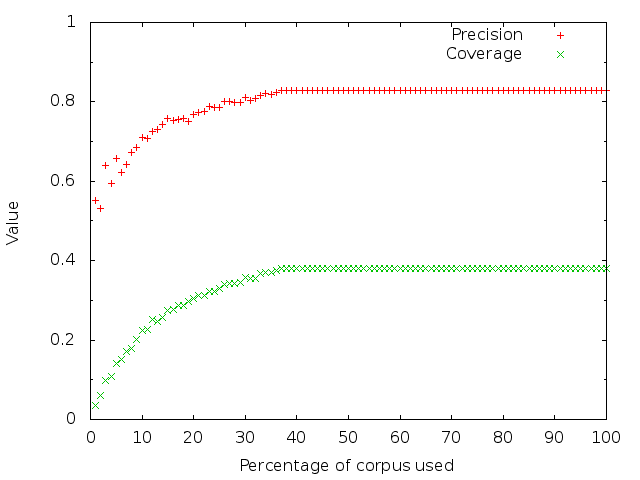
\includegraphics[width=0.45\textwidth]{fig/slot-predicate-percents.png}
    \caption{\label{fig:fonction_predicate}Performance du modèle fonction-prédicat en entraînant le modèle sur une sous-partie du corpus : de 0 à 100~\%.}
\end{figure}

La correspondance probabiliste a une précision 68.33\% mais une couverture
limitée à 38.33\%. La figure~\ref{fig:fonction_predicate} montre que ce niveau
de performance ne demande pas un gros corpus. C'est un enseignement intéressant
pour deux raisons.

\begin{itemize}

    \item Un corpus de petite taille suffit pour obtenir cette performance, ce
    qui est adapté à des domaines où les corpus même non annotés peuvent être
    petits.

    \item L'algorithme ne fait pas de sur-apprentissage en ayant un biais fort
    et une variance faible, ce qui est souhaitable ici.

\end{itemize}

\subsection{Comparaison avec SEMAFOR}

% TODO scores sont en XX
SEMAFOR \citep{das2014frame} est la référence actuelle en annotation en rôles
sémantiques supervisée : c'est le système qui obtient les meilleurs résultats
sur le corpus full-text de FrameNet 1.5. Une comparaison directe n'est pas
possible :

\begin{itemize}
    \item SEMAFOR annote le corpus FrameNet en frames FrameNet et rôles
FrameNet alors que nous l'annotons en classes VerbNet et rôles VerbNet.
    \item Toutes les parties du discours sont annotées alors que nous nous
concentrons sur les verbes.
    \item Les tâches sont découpées différemment. En effet, SEMAFOR découpe la
        tâche en trois parties :
    \begin{itemize}
        \item identification des prédicats déclencheurs ;
        \item identification des frames FrameNet ;
        \item identification des arguments et annotation en rôles sémantiques.
    \end{itemize}
\end{itemize}

Sur la tâche complète, SEMAFOR obtient un score F1 de XX~\%, score à comparer
avec les XX~\% de notre système tout en gardant les limites ci-dessus en tête. 

Il est intéressant de noter l'importance des données d'entraînement pour
SEMAFOR : pour l'identification des frames FrameNet avec des prédicats de la
vérité-terrain\footnote{les résultats pour des déclencheurs identifiés
    manuellement n'ont été donnés que pour le corpus SemEval, un sous-ensemble
du corpus FrameNet 1.5 complet}, les mêmes modèles grimpent de 74.21~\% à
90.51~\% quand la taille du corpus augmente en passant du corpus SemEval (XXX
phrases) au corpus FrameNet 1.5 (XXX phrases).  De la même manière pour
l'identification des arguments avec des frames FrameNet de la vérité-terrain,
les résultats augmentent de 48.09~\% 68.83~\%. C'est très encourageant pour les
domaines disposant de très gros corpus, mais suggère que d'autres solutions
sont à identifier pour les domaines où de tels corpus ne sont pas disponibles.

\section{Travaux futurs}

Nous avons appliqué ce travail à des domaines spécifiques et variés : football,
réchauffement climatique et informatique (Chapitre~\ref{ch:domainsrl}).

% TODO qu'est-ce qui a déjà été fait ici ?
Nous pensons aussi prendre en compte la similarité entre les remplisseurs déjà
identifiés et les remplisseurs pour lesquels un rôle reste encore à identifier
afin d'améliorer nos modèles de probabilité. En effet, l'information des cadres
de sous-catégorisation est cruciale pour identifier les arguments, mais
l'information sémantique concernant le contenu des remplisseurs est aussi utile
pour déterminer le rôle correct.

Enfin, de la même manière que la prise en compte de la voix passive a amélioré
les résultats, d'autres phénomènes de syntaxe profonde doivent être pris en
compte. La coordination est une autre source commune d'erreur. En effet, quand
deux verbes partagent le même sujet, une analyse syntaxique profonde indique à
chaque fois quel est le sujet profond. Voici deux exemples tirés du corpus
FrameNet :

\begin{itemize}

    \item \textit{You are not fair when you belittle Sheik Bin Baz 's blunder and
        exaggerate the one by Sheik Maqdasi ...}

    \item \textit{Hostile and even friendly nations routinely steal information
        from U.S. companies and share it with their own companies}

\end{itemize}

L'objectif est de traiter ces phénomènes de manière plus générale en intégrant
le système de \cite{ribeyre2013systeme} qui permet de prendre en compte de
nouveaux phénomènes en ajoutant de nouvelles règles au système. Ainsi, les
différents phénomènes seront prise en compte de manière cohérente.

\section{Conclusion}

Nous avons implémenté un système d'annotation en rôles sémantiques basé sur la
connaissance. Nous avons utilisé des outils et des corpus disponibles
publiquement qui rendent notre travail facilement reproductible et facilitent
le travail de comparaison, maintenant et dans le futur. Nous avons commencé à
améliorer le système initial, montrant son potentiel. L'indépendance de
l'approche par rapport au corpus considéré la rend attractive pour annoter des
domaines ne disposant que de peu ou pas de corpus annotés en rôles sémantiques.
